    \section{Project context}  
        \section{Hyperspectral Images}
         \subsection{Description}
         \subsection{Applications} 
         	\subsubsection{Remote Sensing} 
         	\subsubsection{Cancer Detection} 
         \section{Classifiers}
     		\subsection{Concept} 
            \subsection{Unsupervised 		classification}
               \subsubsection{KMeans} 
            \subsection{Supervised classification}
            \subsection{Processing chain for hyperspectral image}
               \subsubsection{PCA (Principal Component     Analysis)} 
               \subsubsection{SVN (Support Vector Machine)}
                 \subsubsection{KNN (K-Nearest Neighbor)}
         \section{Parameterized and Interfaced Synchronous DataFlow MoC} 
             \subsection{PREESM} 
          	
	The work conducted in this thesis focuses on processing hyperspectral images. This chapter explains in detail what they are and the two most widespread processing methods   
	  
   Hyperspectral images are defined as an image that has high spectral as well as spatial  resolution, which means that a pixel does not have just the 3 colors of reflectance's values characteristic of usual images.
   
   Hyperspectral Images (HSI) collects high resolution spectral information gathering hundreds of bands from the ultraviolet to the infra-red range of the electromagnetic spectrum. This information is used to distinguish among the different materials composing the captured scene \cite{lee1987synchronous}.
   
     \begin{figure}[H]
        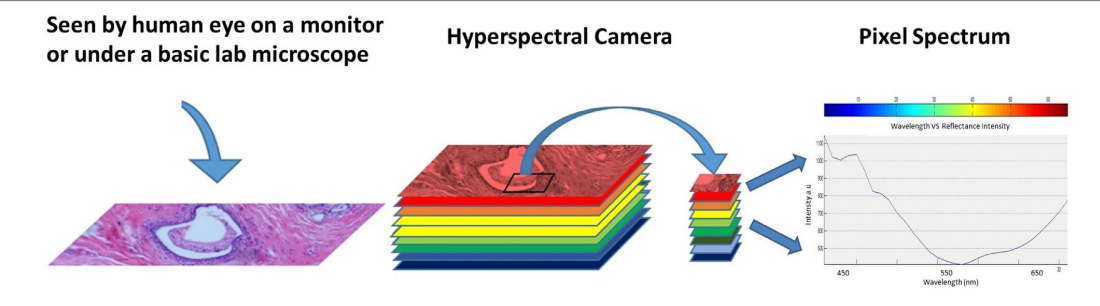
\includegraphics[scale=0.9]{HSI.png}        
        \centering    
        \caption{Comparison between hyperspectral image(left) and RGB image(right)}
        \label{fig:systemArch}
    \end{figure}
       
  
    
  This electromagnetic radiation is not only present among the visible range of wavelengths, as it covers the most part of the electromagnetic spectrum. This kinds of images provide us with useful information as said earlier, as it includes electromagnetic spectrum invisibly to the human eye. However, due to the huge amount of data, processing of HSI images is very computationally expensive.
